\documentclass[border=10pt]{standalone}
\usepackage[svgnames]{xcolor}
\usepackage{amsmath}
\usepackage{pgfplots}
\pgfplotsset{compat=newest}
\usepackage[sfdefault]{FiraSans}
\usepackage{FiraMono}
\renewcommand*\familydefault{\sfdefault}
\begin{document}
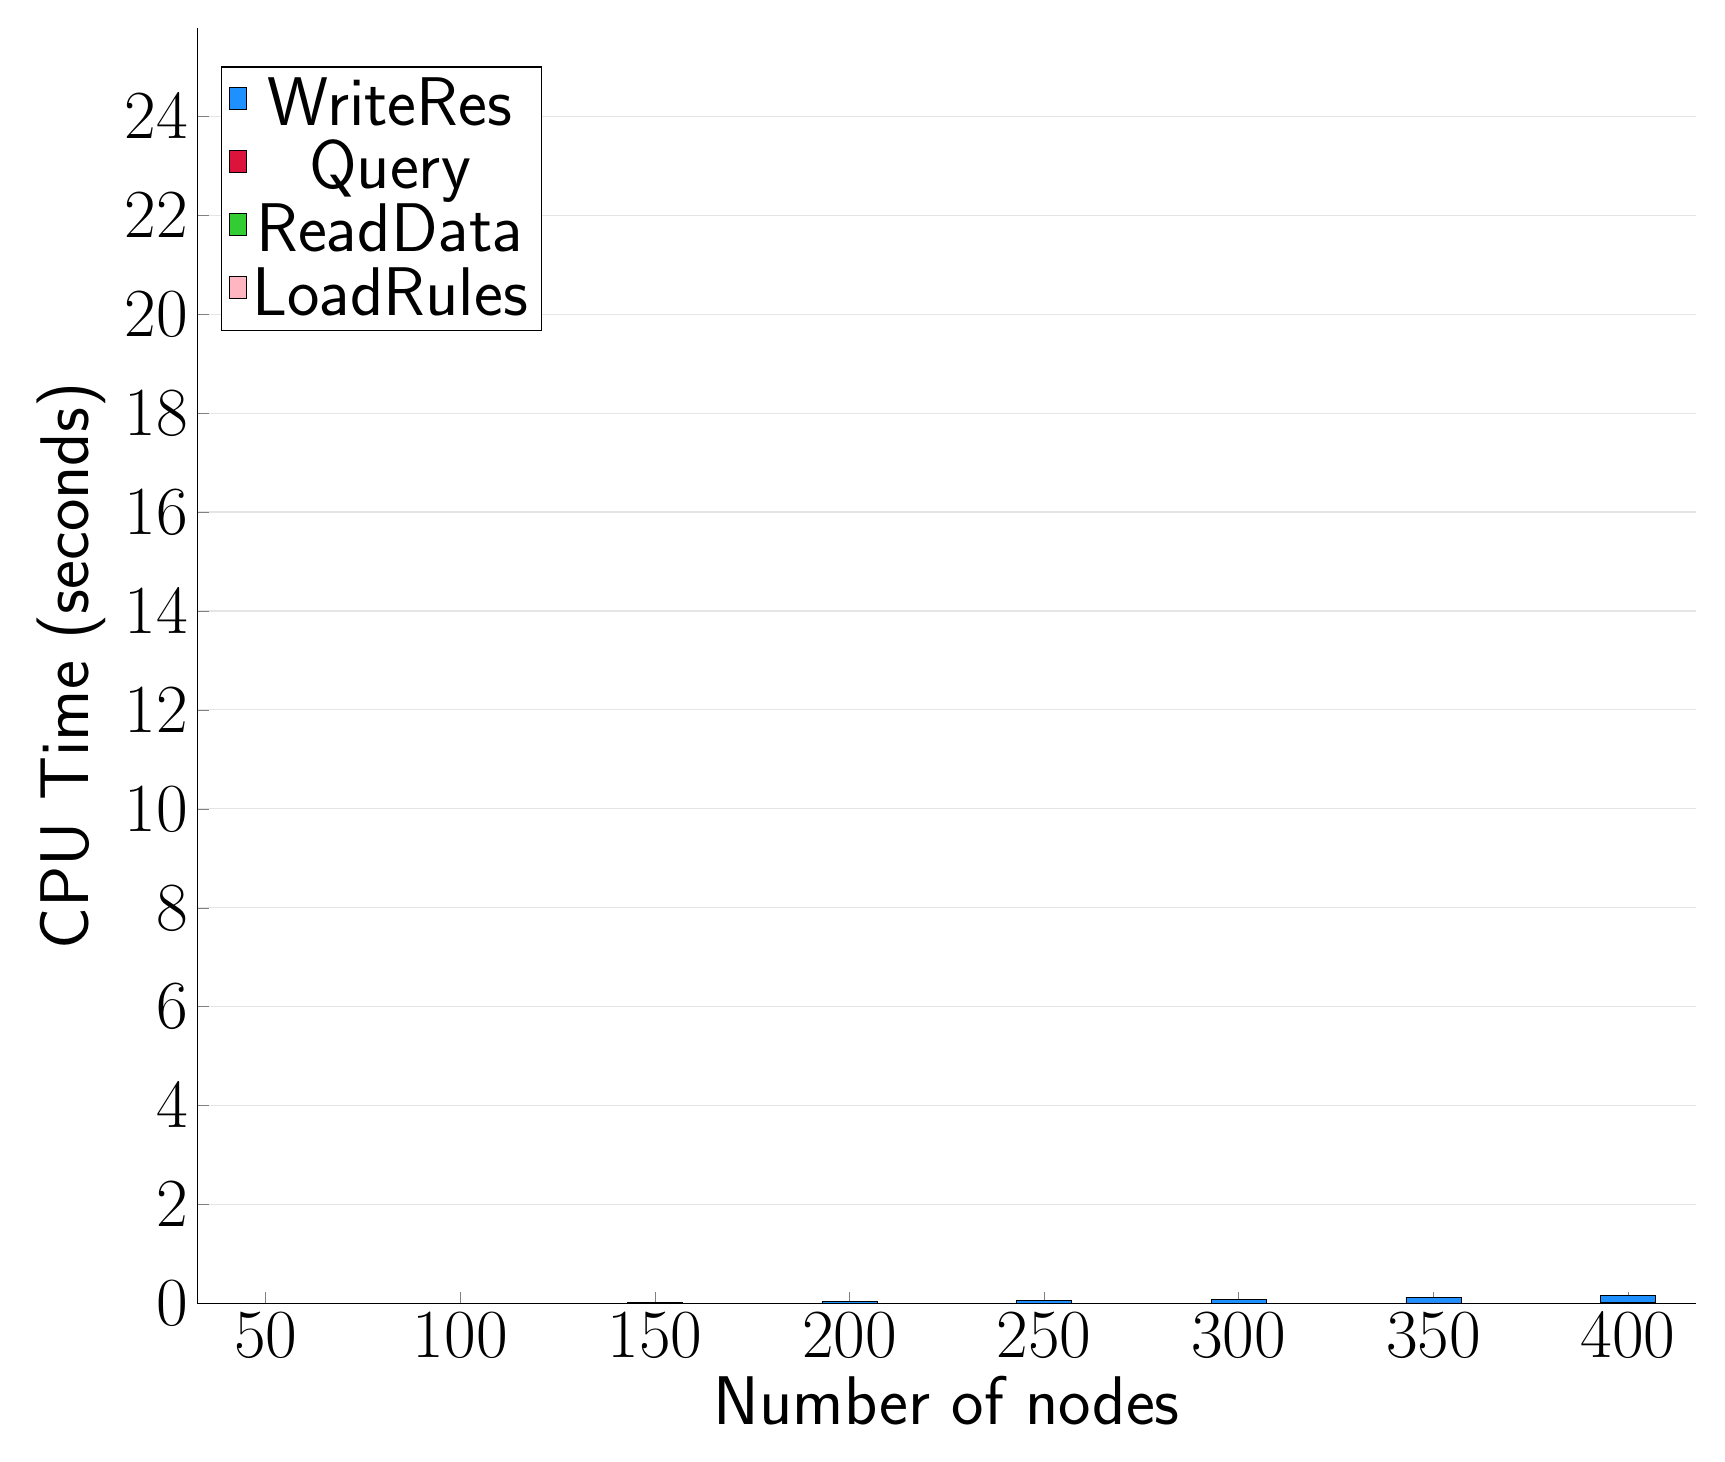
\begin{tikzpicture}
\begin{axis}[
   ybar stacked,
   width=1.7\textwidth,
   bar width=0.7cm,
   ymajorgrids, tick align=inside,
   major grid style={draw=gray!20},
   xtick=data,
   ymin=0, ymax=25.779619999999998,
   axis x line*=bottom,
   axis y line*=left,
   enlarge x limits=0.05,
   legend style={
       at={(0.23, 0.97)},
       anchor=north east,
       legend columns=1,
       font=\Huge,
   },
   ylabel={CPU Time (seconds)},
   xlabel={Number of nodes},
   label style={font=\Huge},
   tick label style={font=\Huge},
]
\addlegendimage{fill=DodgerBlue, draw=black, line width=0.2pt}
\addlegendentry{WriteRes}
\addlegendimage{fill=Crimson, draw=black, line width=0.2pt}
\addlegendentry{Query}
\addlegendimage{fill=LimeGreen, draw=black, line width=0.2pt}
\addlegendentry{ReadData}
\addlegendimage{fill=LightPink, draw=black, line width=0.2pt}
\addlegendentry{LoadRules}
\addplot +[fill=LightPink, draw=black, line width=0.2pt] coordinates {
(50, 0.0006176)
(100, 0.0006015000000000004)
(150, 0.0006180000000000003)
(200, 0.0006121000000000002)
(250, 0.0005969)
(300, 0.0006033)
(350, 0.0006004999999999998)
(400, 0.0006014)
};
\addplot +[fill=LimeGreen, draw=black, line width=0.2pt] coordinates {
(50, 0.0001775000000000002)
(100, 0.0002229999999999999)
(150, 0.0002735999999999999)
(200, 0.0003069999999999998)
(250, 0.0003516000000000004)
(300, 0.00038649999999999996)
(350, 0.0004424999999999999)
(400, 0.0004886000000000001)
};
\addplot +[fill=Crimson, draw=black, line width=0.2pt] coordinates {
(50, 0.00024080000000000008)
(100, 0.0009566000000000005)
(150, 0.0022169)
(200, 0.0038367000000000006)
(250, 0.005970500000000001)
(300, 0.0089801)
(350, 0.013168700000000002)
(400, 0.017085299999999998)
};
\addplot +[fill=DodgerBlue, draw=black, line width=0.2pt] coordinates {
(50, 0.0023085000000000002)
(100, 0.009261599999999998)
(150, 0.0206914)
(200, 0.0369655)
(250, 0.05706019999999999)
(300, 0.083223)
(350, 0.1125246)
(400, 0.1459568)
};
\end{axis}
\end{tikzpicture}

\end{document}
